\documentclass[11pt]{article}
\usepackage[margin=1in]{geometry}
\usepackage{amsmath,amssymb,booktabs,graphicx,hyperref,enumitem,microtype,tikz,algorithmic}
\usetikzlibrary{arrows.meta,positioning}
\hypersetup{colorlinks=true,linkcolor=blue,urlcolor=blue,citecolor=blue}
\title{Anchor-Conditioned Recurrent State-Space World Models for\\
Probabilistic Multi-Asset Realized Volatility Paths}
\author{Tongren Xiao\\\small Independent Researcher}
\date{September 2026}

\newcommand{\RV}{\mathrm{RV}}
\newcommand{\IV}{\mathrm{IV}}
\newcommand{\cF}{\mathcal F}
\newcommand{\TBD}{\textit{pending the formal run}}

\begin{document}
\maketitle

\begin{abstract}
Probabilistic world models promise to represent a latent state and generate future trajectories, but their direct use for financial volatility is difficult. Realized volatility is persistent, non-stationary, heavy-tailed, and exposed to short-lived common shocks. A single stochastic recurrent transition must consequently learn a persistent level, an innovation process, cross-asset dependence, and uncertainty at the same time. We formulate this tension as an identifiable forecasting problem and propose an anchor-conditioned recurrent state-space world model (AC-RSSM). A causal HAR-IV anchor represents the predictable level, while a market-shared and asset-specific RSSM represents residual innovation dynamics. A causal gate modulates the residual mean without mechanically widening its scale. The model is trained on prior-only multi-step residual likelihood, posterior-to-prior consistency, KL balancing, free nats, and gradient clipping. We pre-specify a point-in-time rolling protocol that evaluates point accuracy, marginal calibration, and joint path realism under the same information set. The paper is deliberately written before implementation and formal execution: numerical entries are placeholders until the code is frozen against the equations and the Dow30 run passes the audit protocol.
\end{abstract}

\section{Introduction}

Volatility forecasts are used in risk management, asset allocation, option pricing, and portfolio construction. Realized volatility (RV) is particularly useful because high-frequency returns provide a comparatively informative ex-post measure of intraday variation \cite{andersen2003}. The dominant realized-volatility models, including HAR and its extensions, summarize persistence with lagged daily, weekly, and monthly components \cite{corsi2009}. Implied volatility (IV) adds forward-looking option-market information, while graph-based models use cross-asset spillovers. These models are effective point forecasters, but a point forecast does not specify how a future volatility state evolves or how several assets respond jointly to a common shock.

This paper asks whether a probabilistic world-model formulation can add that missing state and path information. The question is deliberately narrower than building an interactive financial simulator. We study a passive environment in which the information set at the end of day $t$ is used to generate the conditional distribution of the next five daily RV observations:
\begin{equation}
    p(\mathbf{RV}_{t+1:t+H}\mid\cF_t), \qquad H=5.
\end{equation}
The model must therefore satisfy three requirements. First, its state transition must be causal and stable under a prior-only rollout. Second, its samples must preserve path dependence and common movement rather than merely widening independent marginal intervals. Third, any gain attributed to the world model must be incremental relative to the causal HAR-IV anchor, not a consequence of relearning the same persistent level.

The main difficulty became visible in our standard RSSM experiments. Posterior reconstruction of the current observation can be optimized while the prior used at forecast time drifts toward a persistent, low-variance trajectory. Increasing latent noise or adding a shock head can make sampled paths more variable, but it does not necessarily improve the conditional mean of a future shock. This creates a three-way conflict between level accuracy, innovation dynamics, and uncertainty calibration.

We address this conflict with a structured hybrid model. A causal HAR-IV model supplies a level anchor. The RSSM is trained on the residual relative to that anchor and contains a market state shared by all assets and an asset-specific state. A learned market gate modulates only the innovation mean. The predictive scale is estimated separately and is not multiplied by the gate. This decomposition makes the central empirical comparison explicit: if the residual world model has no information beyond the anchor, its out-of-sample loss should be indistinguishable from HAR-IV while its path diagnostics should not improve systematically.

Our contributions are:
\begin{enumerate}[leftmargin=2em]
    \item a causal anchor-conditioned recurrent state-space model for multi-asset RV paths;
    \item a decomposition that separates predictable level, residual innovation mean, and residual uncertainty;
    \item a common point-in-time rolling protocol that evaluates point forecasts, probabilistic calibration, and path realism together;
    \item a falsifiable test of whether stochastic latent innovation adds value beyond a strong HAR-IV level model.
\end{enumerate}

The formal results are intentionally not claimed in advance. In particular, an improvement of AC-RSSM over a pure RSSM would not establish that the RSSM adds value over HAR-IV. The latter is the central ablation in the experiment. The manuscript therefore separates design claims, which are established by the equations and causal protocol, from empirical claims, which remain pending until the pre-specified run is complete.

\begin{figure}[t]
\centering
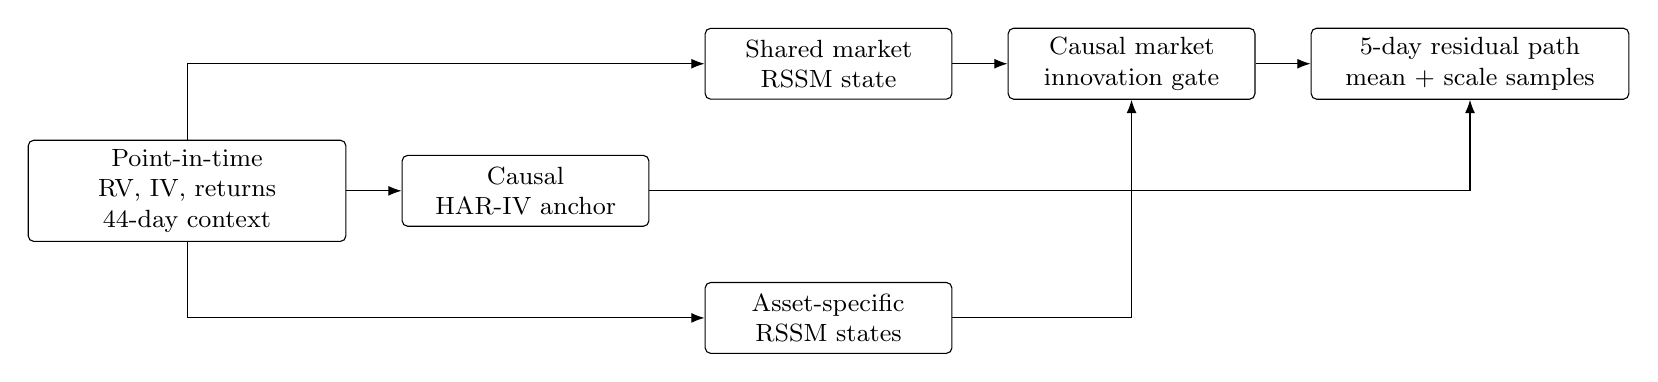
\begin{tikzpicture}[node distance=7mm and 7mm, >=Latex, every node/.style={font=\small},
  box/.style={draw, rounded corners=2pt, align=center, minimum height=9mm, text width=29mm},
  wide/.style={draw, rounded corners=2pt, align=center, minimum height=9mm, text width=38mm}]
  \node[wide] (data) {Point-in-time RV, IV, returns\\44-day context};
  \node[box, right=of data] (anchor) {Causal\\HAR-IV anchor};
  \node[box, above right=of anchor] (market) {Shared market\\RSSM state};
  \node[box, below right=of anchor] (asset) {Asset-specific\\RSSM states};
  \node[box, right=of market] (gate) {Causal market\\innovation gate};
  \node[wide, right=of gate] (path) {5-day residual path\\mean + scale samples};
  \draw[->] (data) -- (anchor);
  \draw[->] (data) |- (market);
  \draw[->] (data) |- (asset);
  \draw[->] (market) -- (gate);
  \draw[->] (asset) -| (gate);
  \draw[->] (anchor) -| (path);
  \draw[->] (gate) -- (path);
\end{tikzpicture}
\caption{Anchor-conditioned passive world model. Level and innovation paths use one causal rolling protocol.}
\label{fig:architecture}
\end{figure}

\section{Related Work}

\paragraph{Realized-volatility forecasting.} HAR uses heterogeneous lag scales to approximate long memory in realized volatility \cite{corsi2009}. The relation between implied and realized volatility motivates IV-augmented specifications \cite{christensen1998}. Multivariate and graph-based models use cross-asset dependence and spillovers; our strongest financial comparator is GNNHAR \cite{zhang2025}. These models define a useful level benchmark but generally produce a conditional mean rather than a joint sample of future paths.

\paragraph{Latent world models.} PlaNet and Dreamer introduced recurrent state-space models in which a posterior state infers observations and a prior transition imagines future states \cite{hafner2019,hafner2025}. DreamerV3 demonstrates that normalization, KL balancing, and robust parameterizations can stabilize latent imagination across many control domains \cite{hafner2025}. Our setting is passive and has no actions, rewards, or policy; the relevant transfer is the separation between inference and prior rollout, not the full reinforcement-learning loop.

\paragraph{Probabilistic time-series dynamics.} Deep latent state-space models can represent stochastic series with sharp transitions \cite{zhou2023}. Recent time-series work separately studies non-stationary dependencies and changing uncertainty. TimeBridge preserves long-run non-stationary relationships while stabilizing short-run dependencies \cite{liu2025}; Non-Stationary Diffusion uses state-dependent location--scale noise for probabilistic forecasts \cite{ye2025}; and D$^3$U separates a deterministic point component from a conditional uncertainty generator \cite{li2025}. These works support our decomposition, but do not establish that a standard RSSM can generate financially realistic multi-asset RV paths.

\section{Forecasting Task and Causal Protocol}

Let $i=1,\ldots,N$ index the fixed Dow30 asset pool and let $v_{i,t}>0$ be daily RV. At forecast origin $t$, the target path is
\begin{equation}
    \mathbf y_t=(\mathbf v_{t+1},\ldots,\mathbf v_{t+H})\in\mathbb R_+^{H\times N}.
\end{equation}
All predictors are measurable with respect to $\cF_t$. We use the common trading-date intersection of RV, IV, and daily returns. RV and IV are log-transformed; returns are clipped to $[-0.25,0.25]$. Standardization parameters are fitted using dates strictly before the first forecast origin of each rolling block. Runtime missing values, if present, are forward-filled only; the upstream ``filled'' files are treated as an external data provenance risk and are not interpreted as a causal audit.

The formal Dow30 run uses dates from the aligned panel, a 44-day context, seven rolling blocks beginning at index 1113 and ending at index 1248, block length 22, one seed (20260721), 600 optimization steps per block, and 500 Monte Carlo paths per origin. The last block is shortened so that all five future targets exist. These values are recorded in `config.yaml` and `manifest.json`.

\section{Anchor-Conditioned World Model}

\subsection{Causal HAR-IV level anchor}

At the beginning of each rolling block with training boundary $b$, we fit a direct regression using observations strictly before $b$:
\begin{equation}
    a_{i,u,h}=\exp\left(x_u^\top\widehat\beta_{i,h}\right),
\end{equation}
where $x_u$ contains an intercept, $v_{i,u-1}$, the mean of $v_{i,u-5:u-1}$, the mean of $v_{i,u-22:u-5}$, and $IV_{i,u-1}$. Coefficients are estimated separately for each asset and horizon using least squares and then frozen throughout the block. Thus the anchor is causal at the deployment boundary: neither validation nor test observations can change its coefficients. This direct daily construction yields an anchor path $\mathbf a_{u,1:H}$.

The model is trained on the standardized log residual:
\begin{equation}
    r_{i,u,h}=\widetilde{\log v}_{i,u+h}-\widetilde{\log a}_{i,u,h}.
    \label{eq:residual}
\end{equation}
This target prevents the latent model from being rewarded for relearning a predictable persistent level that is already represented by the anchor.

\subsection{Market and asset latent states}

At each context date, the market encoder receives six cross-sectional summaries: the mean and standard deviation of standardized log-RV, log-IV, and returns. The market deterministic and stochastic states are $(h_t^m,z_t^m)$; asset $i$ has $(h_{i,t}^a,z_{i,t}^a)$. The context update is
\begin{align}
 h_t^m &= \operatorname{GRU}_m([z_{t-1}^m,\phi_m(o_t)],h_{t-1}^m),\\
 z_t^m &\sim q_m(z_t^m\mid h_t^m,o_t),\\
 h_{i,t}^a &= \operatorname{GRU}_a([z_{i,t-1}^a,o_{i,t},e_i,h_t^m],h_{i,t-1}^a),\\
 z_{i,t}^a &\sim q_a(z_{i,t}^a\mid h_{i,t}^a,o_{i,t},h_t^m),
\end{align}
where $e_i$ is a learned asset embedding. The same market state is supplied to every asset, while each asset retains its own latent state and embedding.

For imagination, the transition removes future observations. It advances the market GRU with a zero observation summary and advances each asset GRU with its previous stochastic state, embedding, and the shared market deterministic state. The prior distributions are
\begin{equation}
    p_m(z_{t+1}^m\mid h_{t+1}^m)=\mathcal N(\mu_{t+1}^m,(\sigma_{t+1}^m)^2),
\end{equation}
and analogously for each asset state.

\subsection{Causal shock gate and residual decoder}

The market gate is
\begin{equation}
    g_t=\operatorname{sigmoid}(f_g([h_t^m,z_t^m]))\in(0,1).
\end{equation}
The residual decoder uses the transitioned states and outputs a mean and scale for each asset. The gate acts only on the residual mean:
\begin{equation}
    \mu^r_{i,t+h}=g_{t+h}\,f_\mu(h_{t+h}^m,z_{t+h}^m,h_{i,t+h}^a,z_{i,t+h}^a,e_i),
\end{equation}
\begin{equation}
    \sigma^r_{i,t+h}=\operatorname{softplus}(f_\sigma(\cdot))+0.05.
\end{equation}
The final sampled path is
\begin{equation}
    \widetilde{\log v}^{(s)}_{i,t+h}=\widetilde{\log a}_{i,t,h}+\mu^r_{i,t+h}+\sigma^r_{i,t+h}\epsilon^{(s)}_{i,t+h},\qquad \epsilon^{(s)}\sim\mathcal N(0,1),
    \label{eq:forecast}
\end{equation}
followed by inverse standardization and exponentiation. The residual is not recursively accumulated on the raw volatility scale; every horizon is anchored to the corresponding causal level forecast.

\subsection{Training objective}

For each sampled training origin, the model maintains a free-running prior state and a teacher-forced state. The prior-only residual NLL is
\begin{equation}
\mathcal L_{\mathrm{free}}=\sum_{h=1}^H\gamma^{h-1}\frac12\left[\left(\frac{r_{t,h}-\mu^r_{t+h}}{\sigma^r_{t+h}}\right)^2+2\log\sigma^r_{t+h}\right].
\end{equation}
The teacher-forced NLL uses the posterior state after observing the actual future observation. The latent regularizer is
\begin{equation}
\mathcal L_{\mathrm{KL}}=\sum_{h=1}^H\gamma^{h-1}\left[\operatorname{KL}(q_m\Vert p_m)+\frac{1}{N}\sum_i\operatorname{KL}(q_{i}^a\Vert p_i^a)\right].
\end{equation}
We also use a small posterior-to-prior mean and log-scale consistency term $\mathcal L_{\mathrm{cons}}$. The total objective is
\begin{equation}
 \mathcal L=\mathcal L_{\mathrm{free}}+0.5\mathcal L_{\mathrm{teacher}}+0.25\max(\mathcal L_{\mathrm{KL}},1.0)+0.05\mathcal L_{\mathrm{cons}},
 \label{eq:loss}
\end{equation}
with $\gamma=0.9$. AdamW, gradient clipping at 100, fixed context length, and fixed seeds are used. No test-period metric is used for training, anchor construction, or hyperparameter selection.

\subsection{Forecasting algorithm}
For clarity, the deployed procedure is fixed before any formal result is inspected. For each rolling block with boundary $b$, (i) fit the HAR-IV anchor using dates strictly before $b$; (ii) fit the RSSM only on context--future tuples whose targets end before the block's test window; (iii) at an origin $t$, encode observations through $t$ and retain the resulting posterior state; (iv) discard future observations and advance the prior transition for $H$ steps; and (v) decode the residual path, add the frozen anchor path, and transform back to the RV scale. In particular, step (iv) never receives $v_{t+1:t+H}$, IV, or returns. The same origins and target dates are then passed to every benchmark.

The resulting computation can be summarized as
\begin{algorithmic}
\STATE Fit $\widehat\beta_b$ on $\{u:u<b\}$ and construct $a_{t,1:H}$.
\STATE Encode $o_{t-L+1:t}$ to obtain $(h_t^m,z_t^m,h_{i,t}^a,z_{i,t}^a)$.
\STATE For $h=1,\ldots,H$: sample the market and asset priors, apply the causal gate, and decode $(\mu^r_{i,t+h},\sigma^r_{i,t+h})$.
\STATE Draw $S$ residual paths and combine each with the corresponding level anchor.
\STATE Store the full path, origin, asset, checkpoint, and information-set hash.
\end{algorithmic}

\subsection{Testable hypotheses}
The decomposition yields three pre-registered hypotheses. H1 (incremental dynamics): conditional on the anchor, AC-RSSM reduces path loss or improves path realism relative to HAR-IV. H2 (dynamic calibration): any improvement is accompanied by a lower gap between predicted and realized increment dispersion and by interval coverage closer to its nominal level. H3 (joint structure): the model improves or preserves the cross-sectional correlation matrix and common-extreme-event coverage. Failure of H1 while H2 or H3 holds is reported as a probabilistic-path result, not as evidence of superior point forecasting. A model is not accepted on the basis of a single metric or a single horizon.

\section{Baselines and Evaluation}

All baselines use the same panel, origins, training boundary, and five-day target path. Naive holds the latest RV constant. HAR uses the three realized-volatility lag components. HAR-IV adds lagged IV. GHAR and GHAR-IV add the contemporaneous cross-sectional mean and dispersion summaries to the same direct regressions. The Hybrid-RSSM is compared with these five baselines. A separate RSSM-only number is not treated as a primary comparison because the model is explicitly trained on the anchor-relative target in Eq.~\eqref{eq:residual}; reporting it without retraining would confound the experiment.

For each horizon $h$, point metrics are MSE, QLIKE, and MAE. For the Hybrid-RSSM samples we additionally report CRPS, 50\% and 90\% coverage, interval width, Winkler score, and rank-PIT mean and variance. Path metrics include the correlation between predicted and realized path increments, the ratio of predicted to realized increment standard deviation, the lag correlation of sampled increments, and the post-shock recovery error. Cross-sectional structure is evaluated with the RMSE between predicted and realized correlation matrices and with common-extreme-event coverage. A date-clustered loss differential provides a descriptive Diebold--Mariano comparison; block bootstrap intervals are reported when enough dates are available.

\section{Formal Experiment}

\subsection{Data and reproducibility}

The included Dow30 archive contains 30 assets and 1,254 common trading dates after intersecting the RV, IV, and return files. The exact dates, tickers, upstream-fill audit, configuration, environment, and code hash are written to `manifest.json`. Each block stores its checkpoint, training history, compressed samples, predictions, and completion status. The command used for the formal run is:
\begin{verbatim}
python -m empirical_runs.world_model_v1.evaluate \\
  --config empirical_runs/world_model_v1/config.yaml
\end{verbatim}

\subsection{Results}

The numerical results are populated only after the formal command completes and the audit script passes. This separation is intentional: pilot smoke runs verify tensor and file contracts but are not evidence of forecast performance.

\begin{table}[ht]
\centering
\caption{Dow30 point-forecast losses. Formal results will be inserted from `summary.csv`.}
\label{tab:point}
\resizebox{\linewidth}{!}{\begin{tabular}{lrrrrrr}
\toprule
Model & MSE$_1$ & QLIKE$_1$ & MSE$_5$ & QLIKE$_5$ & MAE$_1$ & MAE$_5$\\
\midrule
Naive & \TBD & \TBD & \TBD & \TBD & \TBD & \TBD\\
HAR & \TBD & \TBD & \TBD & \TBD & \TBD & \TBD\\
HAR-IV & \TBD & \TBD & \TBD & \TBD & \TBD & \TBD\\
GHAR & \TBD & \TBD & \TBD & \TBD & \TBD & \TBD\\
GHAR-IV & \TBD & \TBD & \TBD & \TBD & \TBD & \TBD\\
Hybrid-RSSM & \TBD & \TBD & \TBD & \TBD & \TBD & \TBD\\
\bottomrule
\end{tabular}}
\end{table}

\begin{table}[ht]
\centering
\caption{Hybrid-RSSM probabilistic and path diagnostics. Formal results will be inserted from `diagnostics.csv`.}
\label{tab:prob}
\resizebox{\linewidth}{!}{\begin{tabular}{lrrrrrr}
\toprule
Horizon & CRPS & Cov.90 & Cov.50 & Width90 & PIT mean & Inc. SD ratio\\
\midrule
1 & \TBD & \TBD & \TBD & \TBD & \TBD & \TBD\\
2 & \TBD & \TBD & \TBD & \TBD & \TBD & \TBD\\
3 & \TBD & \TBD & \TBD & \TBD & \TBD & \TBD\\
4 & \TBD & \TBD & \TBD & \TBD & \TBD & \TBD\\
5 & \TBD & \TBD & \TBD & \TBD & \TBD & \TBD\\
\bottomrule
\end{tabular}}
\end{table}

\section{Discussion and Limitations}

The central empirical question is not whether a stochastic model can be made more variable. It is whether the latent innovation adds conditional information after the persistent level has been removed. A Hybrid gain over a pure RSSM is therefore insufficient; the decisive comparison is Hybrid-RSSM versus HAR-IV under identical origins and training boundaries. Conversely, a failure to improve MSE does not automatically make the world-model formulation useless if it produces better calibrated joint paths, but such a claim requires the path diagnostics and a downstream risk task to support it.

This study has several limitations. The environment is passive and has no actions or market feedback. The experiment uses one Dow30 panel and one seed in the default configuration; seed and universe expansion are required before a strong generalization claim. The source files are labelled as filled upstream data, and their imputation process is not independently audited here. The Gaussian residual distribution may be inadequate for extreme tails. Finally, the five-day horizon is useful for a controlled first study but does not establish long-horizon financial simulation.

\section{Conclusion}

We formulate realized-volatility forecasting as a passive probabilistic world-model problem rather than only a point-regression problem. The proposed architecture assigns persistent level prediction to a causal HAR-IV anchor and assigns short-run stochastic dynamics to a market/asset RSSM with a causal innovation gate. The accompanying protocol tests accuracy, calibration, and path realism separately. The formal Dow30 run will determine whether this decomposition provides an independent gain beyond HAR-IV or instead serves mainly as a useful diagnostic of where world-model assumptions fail in financial volatility.

\begin{thebibliography}{99}
\bibitem{andersen2003} Andersen, T. G., Bollerslev, T., Diebold, F. X., and Labys, P. (2003). Modeling and forecasting realized volatility. \emph{Econometrica}, 71(2), 579--625. \href{https://doi.org/10.1111/1468-0262.00418}{doi:10.1111/1468-0262.00418}.
\bibitem{corsi2009} Corsi, F. (2009). A simple approximate long-memory model of realized volatility. \emph{Journal of Financial Econometrics}, 7(2), 174--196. \href{https://doi.org/10.1093/jjfinec/nbp001}{doi:10.1093/jjfinec/nbp001}.
\bibitem{christensen1998} Christensen, B. J., and Prabhala, N. R. (1998). The relation between implied and realized volatility. \emph{Journal of Financial Economics}, 50(2), 125--150. \href{https://doi.org/10.1016/S0304-405X(98)00034-8}{doi:10.1016/S0304-405X(98)00034-8}.
\bibitem{zhang2025} Zhang, C., Pu, X., Cucuringu, M., and Dong, X. (2025). Forecasting realized volatility with spillover effects: Perspectives from graph neural networks. \emph{International Journal of Forecasting}, 41, 377--397. \href{https://doi.org/10.1016/j.ijforecast.2024.09.002}{doi:10.1016/j.ijforecast.2024.09.002}.
\bibitem{hafner2019} Hafner, D., Lillicrap, T., Ba, J., and Norouzi, M. (2019). Dream to control: Learning behaviors by latent imagination. \emph{International Conference on Learning Representations}. \href{https://arxiv.org/abs/1912.01603}{arXiv:1912.01603}.
\bibitem{hafner2025} Hafner, D., Pasukonis, J., Ba, J., and Lillicrap, T. (2025). Mastering diverse domains through world models. \emph{Nature}, 640, 647--653. \href{https://doi.org/10.1038/s41586-025-08744-2}{doi:10.1038/s41586-025-08744-2}.
\bibitem{zhou2023} Zhou, L., Poli, M., Xu, W., Massaroli, S., and Ermon, S. (2023). Deep latent state space models for time-series generation. \emph{Proceedings of ICML}, 202, 42625--42643. \href{https://proceedings.mlr.press/v202/zhou23i.html}{PMLR}.
\bibitem{liu2025} Liu, P., Wu, B., Hu, Y., Li, N., Dai, T., Bao, J., and Xia, S.-T. (2025). TimeBridge: Non-stationarity matters for long-term time series forecasting. \emph{Proceedings of ICML}, 267, 39815--39840. \href{https://mlanthology.org/icml/2025/liu2025icml-timebridge/}{ML Anthology}.
\bibitem{ye2025} Ye, W., Xu, Z., and Gui, N. (2025). Non-stationary diffusion for probabilistic time series forecasting. \emph{Proceedings of ICML}, 267, 72112--72130. \href{https://mlanthology.org/icml/2025/ye2025icml-nonstationary/}{ML Anthology}.
\bibitem{li2025} Li, Q., Zhang, Z., Yao, L., Li, Z., Zhong, T., and Zhang, Y. (2025). Diffusion-based decoupled deterministic and uncertain framework for probabilistic multivariate time series forecasting. \emph{Proceedings of ICLR}. \href{https://mlanthology.org/iclr/2025/li2025iclr-diffusionbased/}{ML Anthology}.
\end{thebibliography}

\end{document}
